\documentclass[11pt, twoside, a4paper]{book}

\usepackage{graphicx}
\usepackage[utf8]{inputenc}
\usepackage{ngerman}
%\usepackage{lineno}
\usepackage{verbatim}
\usepackage[squaren]{SIunits}
\usepackage{amsmath}
\usepackage{amsfonts}
\usepackage{amssymb}
\usepackage{enumitem}
\usepackage{fancyhdr}
\usepackage{textcomp}
\usepackage{subcaption}
\usepackage[noadjust]{marginnote}
\usepackage{tikz}
\usepackage{nicefrac}
\usepackage{framed}
\usepackage{import}
\usepackage{caption}

\usetikzlibrary{calc,intersections}
\usetikzlibrary{arrows}
\usetikzlibrary{decorations.markings}
\usetikzlibrary{decorations.pathreplacing}
\usepackage[european resistors]{circuitikz}
\usepackage[ 
    top=2cm, 
    bottom=2cm, 
    outer=3cm, 
    inner=3cm,
    marginparwidth=2.5cm,
		headheight=14pt
  ]{geometry}

\usepackage{parskip}
\usepackage{pdfpages}

\newcommand{\Ohm}{$\mathrm\Omega\;$}

\setlength{\parindent}{0pt}

\newcommand{\experimentheader}[4]
{
  \iftutor{{\bf Schwierigkeitsgrad:} #1\\}
  \iftutor{{\bf Dauer:} #2\\}
  {\bf Ger\"ate:} #3\\
  {\bf Bauteile:} #4
}

\newcommand{\hintboxNone}{0}
\newcommand{\hintboxExclamation}{1}
\newenvironment{hintbox}[4][\hsize]
{
  \def\FrameCommand
  {%
    {\color{#3}\vrule width 3pt}%
    \hspace{0pt}%must no space.
    \fboxsep=\FrameSep\colorbox{#4}%
  }%
  \MakeFramed{\hsize#1\advance\hsize-\width\FrameRestore}%
  \mbox{\textbf{#2}:}%
}
{
  \endMakeFramed
}
\newcommand{\xhintbox}[3]
{
  \begin{hintbox}{Achtung}{red!50}{red!10}
    #3
  \end{hintbox}
}

\newenvironment{hint}
{
  \begin{hintbox}{Hinweis}{green!50}{green!10}
}
{
  \end{hintbox}
}

\newenvironment{definition}
{
  \begin{hintbox}{Definition\\}{white!50}{white!10}
}
{
  \end{hintbox}
}

\newenvironment{important}
{
  \begin{hintbox}{Hinweis}{gray!50}{gray!10}
}
{
  \end{hintbox}
}

\newenvironment{jason}
{
  \begin{hintbox}{Achtung}{red!50}{red!10}
}
{
  \end{hintbox}
}

\newcommand{\mandatoryenumi}
{
  \renewcommand{\labelenumi}{\arabic{enumi}.} 
}
\newcommand{\optionalenumi}
{
  \renewcommand{\labelenumi}{$\bigstar$\quad\arabic{enumi}.} 
}
\newcommand{\mandatoryenumii}
{
  \renewcommand{\labelenumii}{(\alph{enumii})} 
}
\newcommand{\optionalenumii}
{
  \renewcommand{\labelenumii}{$\bigstar$\quad(\alph{enumii})} 
}
\newcommand{\icname}[1]{\mbox{\tt #1}}


  \newcommand{\iftutor}[1]{}
\newcommand{\ifnotutor}[1]{#1}

  %\newcommand{\iftutor}[1]{#1}
\newcommand{\ifnotutor}[1]{}


\newenvironment{tutorhint}{\comment}{\endcomment}
\newenvironment{todo}{\comment}{\endcomment}
\newenvironment{solution}{\comment}{\endcomment}
\iftutor
{
  \renewenvironment{todo}
  {
    \hintbox{Todo}{red!50!yellow!90}{red!50!yellow!20}
  }
  {
    \endhintbox
  }
  \renewenvironment{tutorhint}
  {
    \hintbox{Tutorenhinweis der Stunde}{blue!50}{blue!10}
  }
  {
    \endhintbox
  }
  \renewenvironment{solution}
  {
    \hintbox{L\"osung}{black!80}{black!5}
  }
  {
    \endhintbox
  }
}
\newcommand{\etutorhint}[1]
{
  \iftutor{
    \tutorhint
      #1
    \endtutorhint
  }
}
\newcommand{\esolution}[1]
{
  \iftutor
  {
    \solution
    #1
    \endsolution
  }
}
\newcommand{\etodo}[1]
{
  \iftutor
  {
    \todo
    #1
    \endtodo
  }
}



\begin{document}

\renewcommand{\thechapter}{\arabic{chapter}}
\setcounter{chapter}{20}
\def\chaptername{Versuch}

\chapter{Signalausbreitung auf Leitern}
\label{vn:1}

In diesem Versuch lernen Sie die Grundlagen der Ausbreitung von Signalen in elektrischen Netzwerken, wie z. Bsp. elektrischen Leitungen oder Nervenzellen.

%\noindent
%{\bf Kenntnisse}: ???

%------------------------------------------------
\section{Stichworte}
%------------------------------------------------
Spannung, Strom, Ohm'scher Widerstand, Ohm'sche Gesetze, Kirchhoff'sche Regeln, Parallel- und Reihenschaltung von Widerständen
%
%------------------------------------------------
\section{Literatur}
%------------------------------------------------
Gehrtsen, Kapitel 6.1.2, 6.3.1 - 6.3.4
%
%------------------------------------------------
\section{Anwendungsbeispiele}
%------------------------------------------------
%
Anwendungsbeispiele aus der Physiologie finden Sie später in diesem Kapitel.
%
%------------------------------------------------
\section{Theoretischer Hintergrund}
%------------------------------------------------

\subsection{Elektrische Ladung}

Die elektrische \textit{Ladung} ist eine physikalische Eigenschaft von Körpern und hat als Einheit das Coulomb, $ [Q]~=~C$. Diese Ladung kann positive oder negative Werte annehmen und tritt immer in ganzzahligen Vielfachen der kleinsten frei vorkommende Ladungsmenge, der sogenannten \textit{Elementarladung} $e~=~1,6\cdot 10^{-19}~C$, auf. Zum Beispiel hat das Elektron eine Ladung von $Q_e~=~-1\cdot e$, das Proton trägt eine Ladung von $Q_p~=~+1\cdot e$.

\noindent
Normalerweise besitzen Atome genauso viele Elektronen in der Hülle, wie positive Ladungen im Kern. Dann bezeichnet man sie als elektrisch neutral. Ändert sich die Anzahl der Elektronen, so ist das Atome nach außen hin elektrisch geladen und wird dann als \textit{Ion} bezeichnet. Ein Natriumatom, dem ein Elektron fehlt, ist einfach positiv geladen und wird mit Na$^+$-Ion bezeichnet. Die Ladung eines Ions kann auch mehrfach positiv oder negative sein, z.B. Ca$^{2+}$.

\subsection{Spannung, Strom und Widerstand}

Die elektrische \textit{Spannung} ist die Differenz der Coulombpotenziale an zwei Orten, zum Beispiel zwei Punkten in einem elektrischen Schaltkreis:
\begin{equation}
	U = \Phi_A - \Phi_B
\end{equation}
Wie man an dieser Definition sieht, bezieht sich die Angabe einer Spannung immer auf ein Referenzpotenzial, welches entweder explizit angegeben wird (''Spannung zwischen Punkten A und B'') oder impliziert wird (typischerweise die sogenannte ''Erde''). Daher kann eine Spannung \textit{positiv} oder \textit{negativ} sein, je nachdem ob das Potenzial am beschriebenen Punkt höher oder niedriger als das Referenzpotenzial ist. Bei einer Spannungsquelle in einem elektrischen Schaltkreis nennt man den Anschluss mit dem höheren Potenzial den \textit{Pluspol} und den mit dem niedrigeren Potenzial den \textit{Minuspol}. Bei den Schaltsymbolen in den nachfolgenden Schaltplänen bezeichnet der längere Strich an der Spannungsquelle den Pluspol.\\
Diese Potenzialdifferenz erzeugt ein elektrisches Feld ($\vec{E} = -\mathrm{grad}\Phi$), welches auf geladene Teilchen eine \textit{Coulombkraft} in Richtung der Feldlinien ausübt und diese damit beschleunigt. Negativ geladene Elektronen werden dabei auf den Pluspol zu beschleunigt. Die resultierende \textit{Drift} der Ladungsträger, zum Beispiel in einem Draht, nennt man dann \textit{Strom}:
\begin{equation}
	I = \frac{dQ}{dt}
\end{equation}
Die \textit{technische Stromrichtung} ist so definiert, dass Strom vom Pluspol einer Spannungsquelle zum Minuspol fließt (also entgegen der Driftrichtung von Elektronen). In den nachfolgenden Schaltplänen ist teilweise die technische Stromrichtung durch Pfeile gekennzeichnet.\\

\noindent
Die Einheiten von Spannung, $[U]~=~1~V$, und von Strom, $[I]~=~1~A$, das Volt und das Ampere, sind SI Einheiten. \\

\noindent
Der ohmsche Widerstand eines Leiters ist definiert durch das Ohm'sche Gesetz
\begin{equation} \label{eq:Ohm}
R:=\frac{U}{I}\, ,
\end{equation}
seine Einheit $[R]~=~1$~\Ohm\, ist das \textit{Ohm}.

\subsection{Einfache Netzwerke}

Elektrische Netzwerke bestehen aus elektrischen Bauteilen, welche miteinander verbunden werden. In diesem Versuch wollen wir uns mit dem einfachsten passiven Bauteil beschäftigen: dem rein ohmschen Widerstand.\\
Netzwerke sind aus \textit{Knoten} und \textit{Maschen} aufgebaut. Aufbauend auf der Erhaltung der elektrischen Ladung ($\frac{dQ}{dt} = 0$) kann man das Verhalten von Strom und Spannung durch die \textit{Kirchhoffschen Gesetze} beschreiben:\\

\noindent
1. Kirchhoffsches Gesetz (Knotenregel): \\
	Die Summe aller Ströme, die in eine Knoten hinein bzw. aus einem Knoten herausfließen, ist null.
 \begin{equation}
  \sum^n_{k=1}{I_k} = 0 \; .
  \label{eq:Kirchhoff1}
 \end{equation}
%
2. Kirchhoffsches Gesetz (Maschenregel): \\
	Die Summe aller Spannungen in einer Masche ist null.
\begin{equation}
 \sum^n_{k=1}{U_k} = 0 \; .
 \label{eq:Kirchoff2}
\end{equation}

\noindent
Die Kirchhoffschen Gesetze können benutzt werden, um den Strom durch ein Bauteil und die über ihm abfallende Spannung zu beschreiben. Ein Beispiel ist die Berechnung des Gesamtwiderstandes einer Parallel- oder Serienschaltung von Widerständen.
%
\subsection{Parallelschaltung}

\begin{minipage}{0.35\textwidth}
 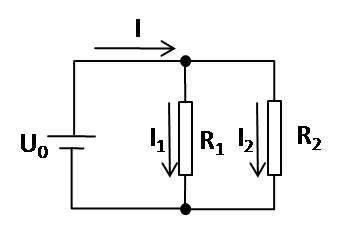
\includegraphics[width=1.00\textwidth]{figures/Parallel.jpg}
 \label{fig:Parallel}
\end{minipage}
%
\begin{minipage}{0.6\textwidth}
Aus der Knotenregel folgt: \hfill $I = I_1 + I_2\, .$\\
Mit dem Ohm'schen Gesetz folgt: \hfill $\frac{U_0}{R_{ges}} = \frac{U_0}{R_1} + \frac{U_0}{R_2}\, .$\\
Den Gesamtwiderstand der Parallelschaltung von Widerständen kann man also schreiben als: 
\begin{equation}
\frac{1}{R_{ges}} = \frac{1}{R_1} + \frac{1}{R_2} = \sum_i{\frac{1}{R_i}} \, .
\end{equation}
\end{minipage}
%
\subsection{Serienschaltung}

\begin{minipage}{0.35\textwidth}
 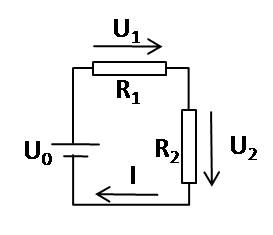
\includegraphics[width=1.00\textwidth]{figures/Seriell.jpg}
 \label{fig:Seriell}
\end{minipage}
%
\begin{minipage}{0.6\textwidth}
Aus der Maschenregel folgt: \hfill $U_0 = U_1 + U_2\, .$\\
Mit Ohm's Gesetz folgt: \hfill $I\cdot R_{ges} = I\cdot R_1 + I\cdot R_2\, .$\\
Den Gesamtwiderstand der Serienschaltung von Widerständen kann man also schreiben als: 
\begin{equation}
R_{ges} = R_1 + R_2 = \sum_i{R_i} \, .
\end{equation}
\end{minipage}
%
\subsection{Der (unbelastete) Spannungsteiler} \label{sec:Spannungsteiler}

In Schaltung \ref{fig:Seriell} kann man die Spannung $U_2$, die über den Widerstand $R_2$ abfällt auch als Eingangsspannung für eine daran anschliessende Schaltung benutzen. Schaltung \ref{fig:Seriell} bezeichnet man in diesem Fall als \textit{Spannungsteiler}. Die Spannung $U_2$ wird dann durch die \textit{Spannungsteilerformel} gegeben, die wir kurz herleiten wollen:\\
Fließt ein Strom $I$ durch $R_2$, so fällt über den Widerstand die Spannung ab
\begin{equation*}
U_2 = I\cdot R_2\; .
\end{equation*}
Aus der Maschenregel folgt für den Strom:
\begin{equation*}
I = \frac{U_0}{R_1 + R_2} \; .
\end{equation*}
Einsetzen ergibt die Spannungsteilerformel:
\begin{equation}\label{eq:Spannungsteiler}
U_2 = U_0\cdot\frac{R_2}{R_1+R_2}
\end{equation}

\subsection{Anwendungsbeispiel: Nervenleitung}

\subsubsection{Spannungsabhängigkeit von Ionenkanälen}

Im Intra- und Extrazellularraum einer Nervenzelle liegen Ionen in unterschiedlicher Konzentration vor. Dieser Unterschied macht sich als Spannung von $U\approx -70$~mV bemerkbar und kann mittels der Nernst-Gleichung berechnet werden. Diese Spannung wird meist als Membranpotenzial bezeichnet, was physikalisch nicht richtig ist, da es sich eigentlich um eine Potenzialdifferenz handelt.\\

\noindent
Die Membran einer Nervenzelle trennt die Elektrolyte im Interzellularraum von denen im Extrazellularraum. Des Weiteren enthält die Membran Ionenkanäle, durch die ein Ionenaustausch stattfinden kann. Wenn kein Ionenaustausch stattfindet stellt sich das oben erwähnte Membranpotenzial von $U\approx -70$~mV ein. Wenn sich diese Spannung zu positiveren Werten verändert (z.B. $U\approx -30$~mV), spricht man von einer Depolarisation, im umgekehrten Fall von einer Repolarisation oder Hyperpolarisation.

\noindent
Ein offener Ionenkanal verhält sich ungefähr wie ein ohm'scher Widerstand: Solange nur die Membranpotenzial von $U\approx -70$~mV an der Membran anliegt, fließt kein Strom. Der Widerstand eines Ionenkanals kann wie in Gleichung \ref{eq:Ohm} gezeigt durch $R=U/I$ berechnet werden. Eigentlich müsste in dieser Gleichung $\Delta U$ stehen, da der Unterschied zum Membranpotenzial entscheidend ist. Zur Vereinfachung wird dieses Potenzial aber meist gleich Null gesetzt, so dass eine Depolarisation einer positiven Spannungsänderung entspricht. Dann kann man das $\Delta$ weglassen.

\noindent
Ionenkanäle zeigen dieses Verhalten nur solange sie geöffnet sind. Wie lange ein solcher Kanal geöffnet ist, hängt von der anliegenden Spannung ab. Bei diesen \textit{spannungsabhängigen Ionenkanälen} wird die Zeitanteil, für den der Kanal geöffnet ist, durch die \textit{Offenwahrscheinlichkeit} angegeben.
\etodo{Plot einfügen}
Wie in Abbildung \textbf{bla} qualitativ für einen Natriumkanal gezeigt ist, bleibt der Kanal für kleine Spannungsänderung fast immer geschlossen. Erst bei einer Depolarisation, wenn das das Membranpotenzial also einen Wert von $U\approx -30$~mV erreicht, nimmt der Zeitanteil im offenen Zustand stark zu. Dies entspricht dem Bereich, in dem eine Nervenzelle ein neues Aktionspotenzial auslöst, da hier die Leitfähigkeit stark ansteigt. Für noch größere Werte des Membranpotenzials geht die Offenwahrscheinlichkeit in Sättigung, da ein Ionenkanal nur für höchsten 75\% der Zeit offen sein kann.

%\noindent
\begin{minipage}{0.4\textwidth}
Um das elektrische Verhalten einer Zellmembran korrekt zu beschreiben, müssen mehrere Ionenkanäle betrachtet werden. Dann kann die Offenwahrscheinlichkeit als der Prozentsatz der Ionenkanäle in offenem Zustand interpretiert werden. Das Verhalten einer Zellmembran kann simuliert werden indem mehrere Widerstände parallel zueinander geschaltet werden. Jeder Widerstand repräsentiert dabei einen offenen Ionenkanal, bei steigender Spannung, i.e. Membranpotenzial, werden also mehr Widerstände parallel geschaltet, bis eine maximale Anzahl erreicht ist, die der Sättigung der Offenwahrscheinlichkeit entspricht. Im Versuch wollen wir die U-I-Kennlinie dieses Modells der Zellmembran vermessen.
\end{minipage}
\hfill
%
\begin{minipage}{0.55\textwidth}
		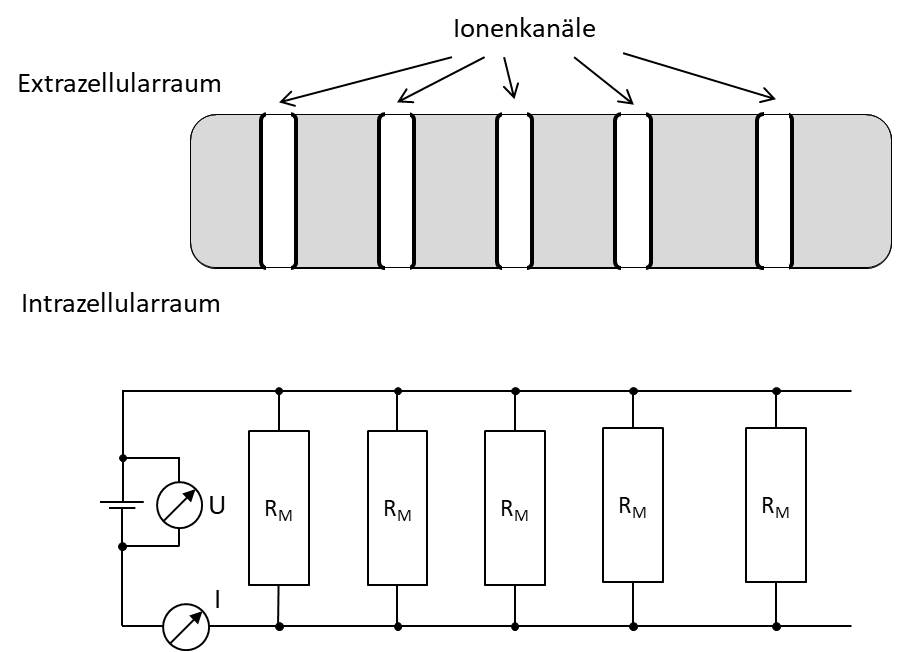
\includegraphics[width=1.00\textwidth]{figures/Membrankanaele.jpg}
	\captionof{figure}{Oben: Abschnitt einer Membran mit mehreren geöffneten spannungsabhängigen Ionenkanälen. Unten: Modell der Membran bei überschwelliger Depolarisation: Alle Ionenkanäle sind geöffnet.}
	\label{fig:Membrankanaele}
\end{minipage}


\subsubsection{Modell der elektrotonischen Erregungsausbreitung}

\begin{figure}[htbp]
	\centering
		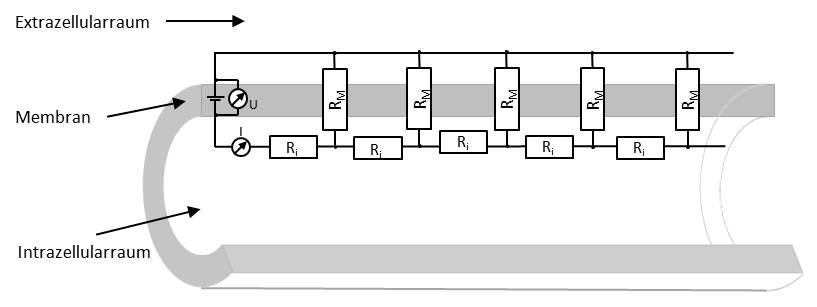
\includegraphics[width=1.00\textwidth]{figures/Axon.jpg}
	\caption{Modell einer langen, dünnen Nervenzelle.}
	\label{fig:Axon}
\end{figure}

In diesem Abschnitt wird neben dem Membranwiderstand auch der Innenwiderstand einer langen, dünnen Nervenzelle, bspw. Axon oder Dendrit, betrachtet. Allerdings können wir, im Gegensatz zum vorigen Abschnitt, nicht die Spannungsabhängigkeit der Ionenkanäle berücksichtigen. Dennoch ergibt sich ein gutes Modell für Zellen mit Membranen, die nur passive Ionenkanäle enthalten, für das Internodium eines myelinisierten Axons oder allgemein für eine unterschwellige Depolarisation an einem Axon.

\noindent
Wie in Abbildung \ref{fig:Axon} dargestellt, kann der Intrazellularraum einer solchen Nervenzelle aufgrund seiner Geometrie mit einem langen, dünnen Leiter verglichen werden. Dieser wird durch den \textit{Innenwiderstand} $R_i$ charakterisiert. Wie jeder elektrische Widerstand ist dieser proportional zur Länge und umgekehrt proportional zur Querschnittsfläche des Leiters. Im Gegensatz zum Inneren der Zelle besitzt der Extrazellularraum keine direkte Begrenzung, so dass die Ionen sich dort relativ frei bewegen können und der elektrische Widerstand damit vernachlässigbar klein ist. Die Stromstärke durch die Membran variiert, je nach Anzahl und Zustand der Ionenkanäle, was durch den Membranwiderstand $R_M$ beschrieben wird.\\
Um das Modell der Zellmembran zu verfeinern, wird dieses typischerweise durch einen Kondensator ergänzt, den wir in diesem Versuch allerdings vernachlässigen werden.\\

\noindent
Im Ruhezustand ist das Membranpotenzial entlang der Membran zunächst überall gleich. Eine Depolarisation, wie sie z.B. bei Reizung sensorischer Nervenzellen erfolgt, breitet sich infolge der frei beweglichen Ionen entlang der Nervenzelle aus. Solange keine aktive Verstärkung des Signals erfolgt, spricht man von passiver oder \textit{elektrotonischer Erregungsausbreitung}.\\
Die elektrotonische Erregungsausbreitung wird durch zwei Größen charakterisiert:
\begin{itemize}
	\item Wie schnell breitet sich die Erregung aus? Dies gibt die sog. Membranzeitkonstante $\tau$ an.
	\item Wie weit kann sich die Erregung entlang der Nervenzelle ausbreiten? Dies wird mit Hilfe der Längskonstante $\lambda$ ausgedrückt.
\end{itemize}
%
Anhand der Schaltung in Abb. \ref{fig:Axon} lässt sich die Abhängigkeit zwischen der an der Membran abfallenden Spannung $U$ und dem Abstand $x$ zum Ursprung der Depolarisation untersuchen.
\begin{itemize}
	\item Die verwendete Spannungsquelle erzeugt einen Strom und verschiebt das Membranpotential. Dies entspricht der Depolarisation. Durch die im Experiment verwendete Gleichspannungsquelle wird eine zeitliche Veränderung der Depolarisation vernachlässigt und der Vorgang ''eingefroren''.
	\item Für den verschwindend geringen Widerstand des Extrazellularraums werden einfache Leitungen, für Innen- und Membranwiderstand die Bauteile $R_i$ und $R_M$ verwendet.
	\item Jeder Abschnitt des Schaltbildes besteht aus einem Innen- und einem Membranwiderstand. Dies entspricht in der Physiologie einem kurzen Abschnitt einer Zellmembran.
\end{itemize}
%
Die Depolarisation führt zu einem Strom im Inneren der Nervenzelle. Wie groß dieser Strom ist, hängt u.a. vom Innenwiderstand $R_i$ ab. Ein Teil des Stroms fließt durch die Ionenkanäle der Membran und über den Extrazellularraum zurück. Die Stärke dieser Leckströme hängt dabei vom Membranwiderstand $R_M$ ab. Aufgrund der Leckströme durch die Membran nimmt der Strom im Intrazellularraum ab. Deshalb nehmen auch die Verlustströme durch die Membran mit der Länge der Nervenfaser, und damit die an den einzelnen Membranwiderständen $R_M$ messbare Spannung ab.\\
Die Abnahme der Depolarisation lässt sich mathematisch über eine Exponentialfunktion beschreiben:
\begin{equation}
	U(x) = U_0\cdot e^{-x/\lambda}
\end{equation}

$U_0$ entspricht dabei für die maximale Depolarisation, die an der Membran am Ort $x=0$ abfällt. Nach der Strecke $x=\lambda$ ist die Depolarisation auf $1/e = 37\%$ ihres Ausgangswertes abgesunken. $\lambda$ ist also ein Maß dafür, wie stark die Depolarisation $U$ mit der Länge $x$ abklingt und wird deshalb als \textit{Längskonstante} bezeichnet.\\

\noindent
Eine dicke Nervenfaser hat aufgrund der großen Querschnittsfläche einen kleinen Innenwiderstand. Daher fließt im Inneren der Nervenzelle ein größerer Strom, der im Vergleich zu dünneren Nervenzellen langsamer mit der Strecke abklingt, und daher die Depolarisation über größere Strecken überschwellig bleibt. Für eine solche Zelle ist der Wert von $\lambda$ größer und die Erregung kann sich weiter ausbreiten.

\noindent
Im Zusammenhang mit ''Saltatorischer Erregungsleitung'' wird häufig davon gesprochen, dass das Signal von Schnürring zu Schnürring springt. Das ist jedoch irreführend, da Ladungen nicht springen können. Bei kontinuierlicher Erregungsleitung am unmyelinisierten Axon werden in sehr kurzen Abständen neue Aktionspotenziale erzeugt, da die Depolarisation ansonsten schnell unterschwellig würde. Das Myelin in den Internodien verhindert dies: Nachdem am Ranvierschen Schnürring ein Aktionspotenzial erzeugt

\begin{tutorhint}
%------------------------------------------------
\section{Fragen zur Vorbereitung}
%------------------------------------------------

\begin{enumerate} 
	\item Wiederholung: Ohm'sches Gesetz, Schaltung von Messgeräten
	%
	\item Wie lauten die Kirchhoff'schen Gesetze? Welche Erhaltungssätze liegen ihnen zugrunde?
	%
	\item Wie berechnet man den Gesamtwiderstand bei Reihen- und Parallelschaltungen von Widerständen?
	%
	\item Wie funktioniert die Spannungsteilerschaltung (Schaltskizze und Erklärung)? 
		\esolution{s. Abschnitt \ref{sec:Spannungsteiler}}
	%
	\item Von welchen Eigenschaften eines Leiters hängt dessen ohm'scher Widerstand ab und wie?
		\esolution{$R=\rho\cdot\frac{A}{L}$ mit dem materialabhängigen spezifischen Widerstand $\rho$, Querschnittsfläche $A$ und Länge $L$.}
	%
	\item In unserem Modell der langen Nervenzelle haben wir die Kapazität der Membran vernachlässigt. Wo würde man diese in der Schaltung in Abb. \ref{fig:Axon} einzeichnen?
		\esolution{Parallel zu $R_M$.}
	%
	\item Wie kommt der Strom innerhalb bzw. ausserhalb der Membran einer Zelle zustande?
		\esolution{Diffusion von Ionen, bspw. K$^+$, Na$^{2+}$, etc. Insbesondere nicht, wie sonst, Drift von Elektronen in einem elektrischen Feld.}
\end{enumerate} 

\end{tutorhint}

%------------------------------------------------
\section{Durchführung} 
%------------------------------------------------
\subsection{Der Spannungsteiler}
\begin{enumerate}
	\item \textbf{Unbelasteter Spannungsteiler}\\
		\begin{minipage}{0.5\textwidth}
			Bauen Sie mit den Bausteinen die nebenstehende Schaltung auf. Benutzen Sie die Widerstandswerte $R_1=R_2=10$~k\Ohm.\\
			Messen Sie die Ausgangsspannung $U_{AB}$ zwischen den Punkten $A$ und $B$ (das Symbol steht für ein Voltmeter) für 5 verschiedene Werte der Eingangsspannung $U_0$.
		\end{minipage}
		%
		\hfill
		\begin{minipage}{0.3\textwidth}
				\begin{figure}[h!]
		\centering
		\begin{circuitikz}
			\begin{scope}[xshift=0cm]
				\draw (2.5,2)
					to [R, i<_=$I$, l=$R_1$](0,2) 
					to [V_=$U_o$] (0,0) 
					to [short] (2.5,0) coordinate (B)
					to [R, l=$R_2$] (2.5,2) coordinate (A);
				\draw (A) to [short, *-o] ++(0.5,0) coordinate (A1);
				\draw (A1) node [anchor=south] {$A$};
				\draw (B) to [short, *-o] ++(0.5,0) coordinate (B1);
				\draw (B1) node [anchor=north] {$B$};
				\draw (B1) to [open, v=$U_{AB}$] (A1);
			\end{scope}
		\end{circuitikz}
		\caption{Spannungsteiler}
		\label{fig:spannungsteiler}
	\end{figure}
		\end{minipage}
	%
	\item Wiederholen Sie die Messung für $R_1=R_2=100$~\Ohm.
	%
	\item \textbf{Belasteter Spannungsteiler}\\	
		\begin{minipage}{0.5\textwidth}
			Erweitern Sie die Schaltung um einen Lastwiderstand $R_L$. Benutzen Sie für diesen verschiedene Widerstandswerte $R_L=51$~\Ohm, 100~\Ohm, 390~\Ohm und 10~k\Ohm.\\
			Messen Sie, bei einer Eingangsspannung $U_0=5$~V, die Ausgangsspannung $U_{AB}$ zwischen den Punkten $A$ und $B$.
		\end{minipage}
		%
		\hfill
		\begin{minipage}{0.4\textwidth}
					\begin{circuitikz}
			\begin{scope}[xshift=0cm]
				\draw (2.5,2)
					to [R, i<_=$I$, l=$R_1$](0,2) 
					to [V_=$U_o$] (0,0) 
					to [short] (2.5,0) coordinate (B)
					to [R, l=$R_2$] (2.5,2) coordinate (A);
				\draw (A) to [short] ++(1,0) coordinate (A1)
					to [R, l=$R_L$] (3.5,0) coordinate (B1)
					to [short] (B);
				\draw (A1) to [short, *-o] ++(0.75,0) coordinate (A2);
				\draw (A2) node [anchor=south] {$A$};
				\draw (B1) to [short, *-o] ++(0.75,0) coordinate (B2);
				\draw (B2) node [anchor=north] {$B$};
				\draw (B2) to [open, v=$U_{AB}$] (A2);
			\end{scope}
		\end{circuitikz}
		\end{minipage}
	%
\end{enumerate}

\subsection{Parallelschaltung von Widerständen oder spannungsabhängige Ionenkanäle}

Jeder geöffnete Ionenkanal wird nun durch einen der Widerstände $R_M=390$~\Ohm ~simuliert. Ein geschlossener Kanal hingegen besitzt einen unendlich hohen Widerstand, daher wird für einen solchen Kanal kein Bauteil verwendet. Die Anzahl der geöffneten Kanäle entspricht also der Anzahl $n$ der parallel geschalteten Widerstände.\\
Um das spannungsabhängige Verhalten der Kanäle zu simulieren, muss die Anzahl der parallel geschalteten Widerstände gezielt variiert werden. 
%
\begin{enumerate}
	\item Bauen Sie jeweils eine Parallelschaltung aus $n$ identischen Widerständen $R_M$ entsprechen Abb. \ref{fig:Membrankanaele} auf und legen Sie die Spannung $U(n)$ gemäß der Vorgaben aus Tabelle \ref{tab:bla} an. Messen Sie jeweils Spannung und Strom. Da es sich um eine Parralelschaltung handelt, kann die Spannung an einem beliebigen Widerstand abgegriffen werden.
	\begin{table*}[h]
	 \centering
		 \begin{tabular}{c||c|c|c|c|c|c|c|c|c|c}
			 n & 1 & 2 & 3 & 4 & 5 & 6 & 7 & 8 & 9 & 10\\ \hline
			 U(n)/V & 0,5 & 1,5 & 2,0 & 2,5 & 2,8 & 2,9 & 3,0 & 3,1 & 3,2 & 3,5
			\end{tabular}
		\caption{Anzahl $n$ parallel geschalteter Widerstände und anzulegende Spannung $U(n)$.}
		\label{tab:bla}
	\end{table*}
	%
	\item Messen Sie für die Parallelschaltung mit 10 Widerständen, i.e. die maximale Offenwahrscheinlichkeit der Ionenkanäle, Strom und Spannung für Spannungen von 4~V bis zur maximalen Ausgangsspannung des Netzteils in Schritten von ungefähr 1~V. Beachten Sie dabei, dass durch den 400~mA Eingang des Multimeters nicht mehr als 400~mA fließen dürfen. Sollte der Strom diesem Wert nahe kommen, wechseln Sie bitte auf die 10~A-Buchsen.
\end{enumerate}

\subsection{Einfache Widerstandsnetzwerke oder elektrotonische Erregungsausbreitung}

\begin{enumerate}
	\item \textbf{Dünne Nervenfaser}\\
	Bauen Sie eine Schaltung wie in Abb. \ref{fig:Axon} dargestellt, mit insgesamt 8 Gliedern. Benutzen Sie die Widerstandswerte $R_M=390$~\Ohm und $R_i=100$~\Ohm. Simulieren Sie eine Depolarisation, indem Sie die maximale Ausgangsspannung des Netzgerätes als $U_0$ anlegen. Messen Sie die Spannung $U_n$, die über jeden der Membranwiderstände $R_M$ abfällt. Schätzen Sie die Unsicherheit der Spannungsmessung ab.
	%
	\item \textbf{Dicke Nervenfaser}\\
	Simulieren Sie die Erregungsausbreitung in einer dicken Nervenfaser, indem Sie die Innenwiderstände durch $R_i=51$~\Ohm Widerstände ersetzen. Messen Sie wieder die Spannungen $U_n$ über die Membranwiderstände.
	%
	\item \textbf{Myelinisierung}\\
	Simulieren Sie die Wirkung des Isolators Myelin, indem Sie die Widerstände durch $R_M=10$~k\Ohm und $R_i=100$~\Ohm ersetzen. Messen Sie wieder die Spannungen $U_n$ über die Membranwiderstände.
\end{enumerate}

%------------------------------------------------
\section{Auswertung} 
%------------------------------------------------
\subsection{Der Spannungsteiler}

\begin{enumerate}
	\item \textbf{Unbelasteter Spannungsteiler}\\
	Tragen Sie die gemessene Ausgangsspannung $U_{AB}$ als Funktion der Eingangsspannung $U_0$ auf und bestimmen Sie die Steigung der Ausgleichsgeraden inkl. deren Unsicherheit. Welche Ausgangsspannung erwarten Sie (bitte kurz mit Formel erläutern)? Stimmt die gemessene Spannung mit Ihrer Erwartung überein?
	%
	\item \textbf{Belasteter Spannungsteiler}\\
	Berechnen Sie für die verschiedenen Widerstandswerte $R_L$ das Verhältnis $U_0/U_{AB}$ und tragen Sie dieses als Funktion des Widerstandes in einen Graphen ein. Was ist der Unterschied zum unbelasteten Spannungsteiler?
\end{enumerate}

\subsection{Parallelschaltung von Widerständen oder spannungsabhängige Ionenkanäle}

Tragen Sie den gemessenen Strom als Funktion der angelegten Spannung $U(n)$ auf. Das ist die sogenannte U-I-Kennlinie der Membran. In welchem Bereich verhält sich die Membran wie ein ohm'scher Widerstand? Wieso tut sie das nur dort?

\subsection{Einfache Widerstandsnetzwerke oder elektrotonische Erregungsausbreitung}

\begin{enumerate}
	\item \textbf{Dünne Nervenfaser}\\
	Tragen Sie die am $n$-ten Glied gemessene Spannung gegen die Zahl $n$ graphisch auf. Lesen Sie aus dem Graphen die Längskonstante $\lambda$ ab und schätzen Sie deren Unsicherheit $\sigma(\lambda)$.
	%
	\item \textbf{Dicke Nervenfaser}\\
	Tragen Sie die am $n$-ten Glied gemessene Spannung gegen die Zahl $n$ im selben Graphen ein. Lesen Sie wieder die Längskonstante $\lambda$ und deren Unsicherheit $\sigma(\lambda)$ ab.
	%
	\item \textbf{Myelinisierung}\\
	Tragen Sie die am $n$-ten Glied gemessene Spannung gegen die Zahl $n$ wieder im selben Graphen ein. Lesen Sie die Längskonstante $\lambda$ und deren Unsicherheit $\sigma(\lambda)$ ab.
\end{enumerate}

\end{document}